\chapter{Implementation}
\label{cha:implementation}

\subsection{Preliminaries}
De kennis over het ISP staat beschreven in een theorie T over een vocabularium $\Sigma$. Dit vocabularium bestaat uit een set $\Sigma\textsubscript{p}$ van predicaatsymbolen en een set van functiesymbolen $\Sigma\textsubscript{f}$. Een interpretatie I bestaat uit D de verzameling domeinelementen, een mapping van elk functiesymbool f/n naar een functie met ariteit n op D en een mapping van elk predicaatsymbool P/n naar een relatie R $\subseteq$ D$\textsuperscript{n}$. Een three-valued parti\"{e}le interpretatie bestaat uit een mapping op drie waarheidswaarden {u,t,f} respectievelijk onbekend, waar en niet waar. De waarheidswaarden zijn partieel geordend volgens precisie, u $\leq\textsubscript{p}$ f en u $\leq\textsubscript{p}$ t. De bedoeling is om een exacte interpetatie te bekomen met maximale precisie die consistent is met de theorie T.

\section{Constructie ISP Theory}

\paragraph{Analyse van het ISP}
Alvorens te beginnen aan het opstellen van een theorie in IDP, is het belangrijk om de regels en structuren van het ISP te bestuderen. Het doel is om een theorie te ontwikkelen die zo algemeen mogelijk is, zodanig dat ze in staat is om een correcte interpretatie te beschrijven voor verschillende opleidingen. En het vinden van structuren, patronen, regels en types die vaak (of altijd) terugkomen, kan in grote mate bijdragen aan zo'n goede theorie. Omdat het onderwijsaanbod aan de K.U. Leuven zodanig groot is, heb ik mijn analyse beperkt tot een kleine groep opleidingen binnen de faculteit Wetenschappen en Ingenieurswetenschappen. Wat meteen opvalt is dat bepaalde types van elementen telkens voorkomen namelijk vakken (meer specifiek de vakcode), studiepunten, fases en semesters. Vakken maken altijd deel uit van een groep, en voor verschillende groepen gelden vaak andere regels. Zulke groepen of anders genoemd \textit{vakGroepen} zijn onderverdeeld in een bepaald type van vakgroep. (elke groep behoort tot \'{e}\'{e}n uniek type) en afhankelijk van het type kunnen er mogelijk nog extra constraints gelden voor een VakGroep. Deze types die steeds terugkomen in meerdere opleidingen hebben ongeacht de opleiding waar ze in voorkomen dezelfde regels die ermee gepaard gaan. Zo is elke opleiding op zich een vakgroep van het type opleiding, het bevat vakken die je verplicht bent te volgen en keuzevakken. Het heeft een minimum (en maximum) aantal studiepunten dat de student verplicht moet opnemen. Een ander belangrijk type vakgroep is de (hoofd)specialisatie, verscheidene opleidingen geven de keuze tussen meerdere specialisaties. Verwacht wordt dat je van minstens \'{e}\'{e}n zo'n specialisatie alle verplichte vakken opneemt. Naast hoofdspecialisatie bestaat er ook het type verdere specialisatie, waarin de student verplicht wordt een bepaald aantal studiepunten op te nemen aan vakken uit deze of bepaalde andere vakgroepen. Vervolgens is er het type 'Algemeen vormende en onderzoeksondersteunende groep' vakgroep, dit is veruit het moeilijkste type groep om te beschrijven. De student moet opnieuw een bepaald aantal studiepunten aan vakken opnemen uit deze groep. Maar daarnaast gelden er ook specifieke regels voor verscheidene vakken die deel uitmaken ervan. En als laatse is er het type 'Bachelor verbredend pakket', waarin studenten die beginnen aan hun masteropleiding vakken moeten opnemen die ontbraken in hun bacheloropleiding. Deze types zien we het vaakst voorkomen en kunnen ongeacht de opleiding met dezelfde set van regels beschreven worden. Het is mogelijk dat sommige types van vakgroepen niet telkens voorkomen, en dus de regels ook niet van kracht zijn. In een bacheloropleiding zal bijvoorbeeld nooit een vakgroep voorkomen van het type Bachelor verbredend pakket. De resultaten van de analyse moeten vervolgens verwerkt worden in een vocabularium dat gebruik maakt van deze types en structuren. Op basis van dat vocabularium hoort dan een theorie ontwikkeld te worden die in staat is een geldige interpretatie voor de verschillende opleidingen te beschrijven. 

\subsection{Vocabularium}
Om te beginnen zal ik de structuur dit vocabularium toelichten, hieronder vallen de types, predicaten en functies.
\subsubsection{Types}
\begin{description}
\item [Vak] Dit type omvat de verzameling van de verschillende vakken in het domein, elke opleiding bestaat uit verschillende vakken die een gebruiker mogelijk kan selecteren. Meer specifiek zijn dit de unieke vakcodes van een vak. De naam van een vak is namelijk niet altijd uniek in tegenstelling tot de vakcode. 
De domeinwaarden zijn niet de naam in natuurlijke taal, maar de unieke vakcode.
\item [VakGroep] Vakken maken altijd deel uit van een groep, en per VakGroep gelden vaak unieke regels. 
\item [VakGroepType] Elke vakGroep maakt deel uit van een bepaald type groep, en per type groep gelden er bepaalde regels bovenop de regels van de individuele groep zelf.
\item [Fase] Opleidingen bestaan uit fases oftewel jaren, de Master Computer Wetenschappen bestaat bijvoorbeeld uit 2 fases. Vakken binnen een opleiding kunnen enkel gevolgd worden tijdens de fase van de opleiding waartoe ze behoren. 
\item [Semester] De K.U. Leuven werkt met een semester systeem, dit wil zeggen dat elke fase (schooljaar) is opgedeeld in twee semesters. Elk vak kan gevolgd worden in de semester waartoe het behoort. Er bestaan ook jaarvakken waarvoor de werklast verdeeld is tussen beide semesters, een voorbeeld hiervan is de Masterproef.
\item [Studiepunten] Ieder vak bevat studiepunten, deze beschrijven de geschatte werklast voor dit vak. Vakgroepen vereisen vaak dat je een bepaalde hoeveelheid een studiepunten opneemt. 
\end{description}

\subsubsection{Predicaten}
De predicaten zijn opgedeeld in twee verzamelingen, de eerste omvat alle predicaten die op voorhand gegeven zijn en waarvan de waarheidswaarde al bekend is. In feite zijn dit de predicaten die de eigenlijke samenstelling van een opleiding uitdrukken. Dit is een lijst van de predicaten die tot deze groep behoren:
\begin{description}
\item [IsType(VakGroep,VakGroepType)] Verzamelingen van vakken (of vakgroepen) behoren altijd tot \'{e}\'{e}n bepaald type. Voor elk type van vakgroep geldig bepaalde regels bovenop de regels de mogelijk van toepassing zijn op de vakgroep zelf. 
\item [InVakGroep(Vak,VakGroep)] Vakken maken altijd deel uit van een bepaalde vakgroep, InVakGroep/2 drukt deze relatie uit. 
\item [InFase(Vak,Fase)] Dit predicaat drukt uit in welke fases van de opleiding een vak gevolgd kan worden, voor elk vak bestaat er minstens \'{e}\'{e}n fase waarin het gegeven wordt. Als de student en vak wil volgen heeft hij/zij de keuze uit \'{e}\'{e}n van deze fases.
\item [Verplicht(Vak,Fase)] Vakken die behoren tot een vakgroep kunnen mogelijk verplicht, m.a.w. de student zal ze moeten opnemen.
\end{description}

De tweede verzameling zijn de predicaten waarvan de waarheidswaarde op voorhand niet gekend is, en waarvan verwacht wordt dat de gebruiker deze stap per stap invult. Hiertoe behoren slechts twee predicaten namelijk Geselecteerd(Vak,Fase) en GeenInteresse(Vak). Geselecteerd/2 geeft aan welke vakken de student wenst op te nemen tijdens de opleiding. GeenInteresse/1 daarentegen is eigenlijk een predicaat waarmee aangegeven kan worden dat een student helemaal geen interesse heeft om een vak te volgen. Dit is vooral handig als de student een geldige selectie wil laten genereren door het systeem waarbij hij/zij op voorhand kan aangeven dat deze selectie zeker niet de vakken kiest waarin de student geen interesse heeft. Het is niet verplicht dat de gebruiker invulling geeft aan dit predicaat. Door aan te geven dat de student geen interesse heeft om een bepaald vak te volgen kan het systeem afleiden dat er geen fases zijn waarin het vak geselecteerd kan worden.

\subsubsection{Functies}
De functies koppelen een bepaald resultaat aan een combinatie van waarden uit het domein. Zo geven de functies MinAantalStudiepunten(VakGroep):Studiepunten en MaxAantalStudiepunten(VakGroep):Studiepunten respectievelijk het minumum en het maximum aantal studiepunten weer dat de student verplicht is te selecteren. Deze relaties zijn gekend op voorhand door het systeem en de student moet uiteraard trachten zich hieraan te houden. GeselecteerdAantalStudiepuntenPerVakGroep(VakGroep):Studiepunten is de relatie tussen het de som van de studiepunten van de vakken die reeds geselecteerd zijn die behoren tot de betreffende vakgroep. Naargelang de selectie kunnen deze waarden verschillen aangezien ze afhankelijk zijn van de keuze van de gebruiker. In het vocabularium zijn meerdere functies terug te vinden die gelijkaardige relaties uitdrukken zoals hierboven beschreven. 


\section{Features}

\subsection{Selectieproces}
Elke keuze die de gebruiker maakt moet zorgvuldig afgehandeld worden om te kunnen geranderen dat de selectie altijd satisfieerbaar is. De voorwaarde is dat als de gebruiker een keuze maakt die ervoor zorgt dat de theorie niet langer satisfieerbaar is, hij hier meteen op de hoogte van wordt gebracht zodanig dat hij dit kan oplossen alvorens verder te gaan. Er wordt gestart met de minst precieze interpretatie W$\textsubscript{0}$ om uiteindelijk stapsgewijs tot een exacte interpretatie W$\textsubscript{n}$ met maximale precisie te komen waarvoor geldt dat W$\textsubscript{n}$ $\cup$ G $\models$ T. Hoe deze stappen verlopen staat beschreven in onderstaand algoritme. Hier wordt W opnieuw opgedeeld in drie verzamelingen U, P en O. U is de verzameling van predicaten met een waarheidswaarde $\geq\textsc{p}$ u, waarvoor geldt dat deze toegekend zijn door de gebruiker. De tweede verzameling P bevat eveneens predicaten met een waarheidswaarde $\geq\textsubscript{p}$ u, maar deze zet zijn de propagaties die volgen uit U. O tenslotte is de set van predicaten waarvoor de waarheidswaarde nog onbekend is. Voor W$\textsubscript{0}$ geldt: W$\textsubscript{0}$ = O$\textsubscript{0}$ en U$\textsubscript{0}$ = P$\textsubscript{0}$ = $\emptyset$. In het verder verloop van de tekst zal deze beschrijving blijven gelden en terugkomen.

\begin{algorithm}
	\SetKwInOut{Input}{Input}
	\SetKwInOut{Output}{Output}
	\underline{function Selectieproces} (U$\textsubscript{i}$)\;
	\Input{De nieuwe keuze van de gebruiker P$\textsubscript{i}$}
	\Output{}
	\eIf{Sat(U$\textsubscript{i}$)}
		{
		V $\leftarrow$ P$\textsubscript{i-1}$ $\cap$ O$\textsubscript{i}$\;
		\eIf{V $\neq$ $\emptyset$}
			{
			V' $\leftarrow$ KeuzeGebruiker(V)\; 
			Selectieproces(U$\textsubscript{i}$ $\cup$ V')\;
			}
			{
			P$\textsubscript{i}$ $\leftarrow$ Propagate(U$\textsubscript{i}$)\;	
			NieuweGebruikerActie(U$\textsubscript{i-1}$,U$\textsubscript{i}$,
			P$\textsubscript{i-1}$,P$\textsubscript{i}$,
			O$\textsubscript{i-1}$,O$\textsubscript{i}$)\;
			}
		}
		{
		N $\leftarrow$ Unsat(U$\textsubscript{i}$)\; 
		K,L $\leftarrow$ ManueleResolutie(N)\;
		U'$\textsubscript{i}$ $\leftarrow$ U$\textsubscript{i}$ 
		[K] - L\; 
		Selectieproces(U'$\textsubscript{i}$)\;
		}
	\caption{Selectieproces}
\end{algorithm}

\subsection{Propagatie}
Bij het samenstellen van een ISP kan het systeem de informatie die de gebruiker reeds verder gaan propageren. Hierbij baseert het systeem zich op de regels van de theorie. Neem het volgende voorbeeld: 
\begin{lstlisting}[mathescape]
Geselecteerd(A) $\Rightarrow$ Geselecteerd(B)
\end{lstlisting}
Deze regel zegt dat als A geselecteerd is, B ook geselecteerd moet zijn. Als de gebruiker A selecteerd, zal het systeem hieruit afleiden dat B ook geselecteerd moet doen. In de GUI zal te zien zijn dat B ook geselecteerd is, hoewel de gebruiker dit niet expliciet heeft gekozen.

\subsection{Model Expansie}
Als de gebruiker al zijn/haar voorkeuren heeft ingevuld in de parti\"{e}le interpretatie W$\textsubscript{i}$ met U$\textsubscript{i}$ $\cup$ P$\textsubscript{i}$ $\cup$ O$\textsubscript{i}$ = W$\textsubscript{i}$ en O$\textsubscript{i}$ $\neq$ $\emptyset$. Dan kan het systeem de verzameling van predicaten O$\textsubscript{i}$ waarvan de waarheidswaarde nog onbekend is, verder oplossen. Om zo tot een interpretatie W$\textsubscript{f}$ to komen met U$\textsubscript{i}$ $\cup$ P$\textsubscript{i}$ $\subseteq$ W$\textsubscript{f}$. W$\textsubscript{f}$ is tevens (precisie )maximaal en W$\textsubscript{f}$ $\cup$ G $\models$ T. Anders gezegd zal het systeem de parti\"{e}le selectie verder vervolledigen tot een geldig ISP. 

\subsection{Minimizatie}
Het is niet alleen mogelijk om een parti\"{e}le selectie verder te laten vervolledigen, maar om hierbij ook een parameter in acht te nemen en een interpretatie W$\textsubscript{f}$ te bekomen waarbij deze parameter zo klein mogelijk is. Het systeem kan een optimalisatie van volgende parameters zoeken:
\begin{itemize}
\item[Werklast] Met werklast wordt bedoeld het aantal studiepunten dat opgenomen wordt. Een student is verplicht vakken te selecteren en gekoppeld aan die vakken zijn studiepunten. De student kan vragen aan het systeem om een ISP samen te stellen waarbij de werklast (de som van de studiepunten van de geselecteerde vakken) ze laag mogelijk is.
\item[Werklast per semester] Vakken die geen jaarvakken zijn, vallen ofwel in het eerste semester of het tweede. Het systeem kan een ISP samenstellen waarbij het verschil in studiepunten tussen geselecteerde vakken van eerste en tweede semester zo klein mogelijk is. Zodat de werklast zo goed mogelijk verdeeld is tussen beide semesters.
\item[Overlap] Vakken hebben uiteraard lesmomenten en het kan al eens gebeuren dat deze lesmomenten voor verschillende vakken samenvallen. Dit is uiteraard niet ideaal voor de student om die niet op twee plaatsen tegelijk kan zijn. Stel dat er het lesmoment van vak A gepland is van 16u tot 18u en het lesmoment voor vak B vindt plaats op dezelfde dag van 15u tot 17u. De overlap bedraagt dan 60 minuten. De student kan een ISP laten genereren waarbij de totale som van alle overlap zo minimaal mogelijk is. 
\end{itemize}

\subsection{Ongedaan Maken}
Het ongedaan kunnen maken van selecties is een van de aspecten waar meerdere strategi\"{e}en mogelijk zijn. Elke stap in het selectieproces (nieuwe selectie door de gebruiker) wordt bijgehouden in een zogenaamde \textit{actie}. Deze actie bevat niet alleen die nieuwe interpretatie W$\textsubscript{i}$ maar ook de voorgaande W$\textsubscript{i-1}$ zodanig dat als en actie ongedaan gemaakt wordt het systeem weet wat de toestand voorheen was en hier naar kan terugkeren. Het is niet noodzakelijk zo dat in een actie A$\textsubscript{i}$ met interpretaties W$\textsubscript{i-1}$ en W$\textsubscript{i}$ dat W$\textsubscript{i-1}$ $\leq\textsubscript{p}$ W$\textsubscript{i}$. Acties beschrijven elke handeling in de tijd gemaakt door de gebruiker, dus ook de waarheidswaarde van een predicaat minder specifiek maken. Ongedaan maken in deze context betekent dus niet automatisch de huidige selectie minder specifiek maken, maar eerder terugkeren in de tijd.

\paragraph{Strategie 1a}
De eerste strategie houdt in dat als een actie ongedaan gemaakt wordt de interpretatie W$\textsubscript{i}$ simpelweg vervangen wordt door de voorgaande W$\textsubscript{i-1}$. Dit is wellicht de meest simpele strategie aangezien er geen extra bewerkingen uitgevoerd moeten worden buiten het terugkeren naar de voorgaande interpretatie.

\begin{algorithm}
	\SetKwInOut{Input}{Input}
	\SetKwInOut{Output}{Output}
	\underline{function MaakActieOngedaan} (Ac)\;
	\Input{De actie die ongedaan gemaakt moet worden A$\textsubscript{i}$}
	\Output{}
	verwijder(A$\textsubscript{i}$)\;
	W$\textsubscript{i}$ $\leftarrow$ W$\textsubscript{i-1}$\;
	\caption{MaakActieOngedaan\label{alg:Strategie1a}}
\end{algorithm}

\paragraph{Strategie 1b}
Bij de voorgaande strategie staat een actie ongedaan maken gelijk aan simpelweg de klok terugdraaien en W$\textsubscript{i}$ vervangen door W$\textsubscript{i-1}$. Dus eventuele propagaties die volgden uit de keuze van de gebruiker in de actie worden ook ongedaan gemaakt. En in plaats van alles simpelweg ongedaan te maken zou het beter zijn als de gebruiker de keuze krijgt om eventuele propagaties te behouden. Dit zorgt echter voor het volgende probleem. De assumptie is dat acties handelingen weergeven in de tijd gemaakt door de gebruiker, het ongedaan maken van handelingen wordt dus gezien als het terugdraaien van de tijd. Maar als de gebruiker kiest om een actie ongedaan te maken en tegelijk eventuele propagaties toch wil behouden dan geldt deze assumptie niet meer. In \ref{alg:Strategie1b} staat beschreven hoe dit probleem opgelost kan worden. Het is simpelweg een uitbreiding op de eerste strategie, een actie wordt nog altijd verwijderd en de laatste interpretatie W$\textsubscript{i}$ wordt vervangen door de voorgaande W$\textsubscript{i-1}$. Maar waar het hier voorheen stopte gebeurt er nu het volgend. Er wordt gecontroleerd of er een set van predicaten V bestaat die zowel toebehoren aan O$\textsubscript{i-1}$ en P$\textsubscript{i}$. Ofwel predicaten waarvoor de waarheidswaarde eerst onbekend was en daarna een meer specifieke waarheidswaarde hebben gekregen d.m.v. propagatie als gevolg van de keuze van de gebruiker. Is deze set niet leeg dan zal de gebruiker moeten kiezen in \emph{KeuzeGebruiker} welke van de propagaties te houden. In het geval dat de gebruik kiest om propagaties te behouden, worden deze niet langer gezien als propagaties maar eerder als keuzes gemaakt door de gebruiker. Deze worden toegevoegd een de verzameling U en dit wordt gezien als een nieuwe handeling in het selectieproces waarvoor een nieuwe actie gecre\"{e}erd zal worden.

\begin{algorithm}
	\SetKwInOut{Input}{Input}
	\SetKwInOut{Output}{Output}
	\underline{function MaakActieOngedaan} (Ac)\;
	\Input{De actie die ongedaan gemaakt moet worden A$\textsubscript{i}$}
	\Output{}
	V $\leftarrow$ O$\textsubscript{i-1}$ $\cap$ P$\textsubscript{i}$\;
	verwijder(A$\textsubscript{i}$)\;
	W$\textsubscript{i}$ $\leftarrow$ W$\textsubscript{i-1}$\;
	\If{V $\neq$ $\emptyset$}
		{
		V' $\leftarrow$ KeuzeGebruiker(V)\;
		\If{V' $\neq$ $\emptyset$} 
			{
			Selectieproces(U$\textsubscript{i-1}$ $\cup$ V')\;
			}
		}
	\caption{MaakActieOngedaan\label{alg:Strategie1b}}
\end{algorithm}

\paragraph{Strategie 2}
Voorheen was de assumptie dat een actie ongedaan maken gelijk stond aan de tijd als het ware terugdraaien en de interpretatie vervangen door de voorgaande. En dat dit niets te maken had met de precisie ordening van de interpretaties. Voor deze strategie wordt er niet meer uitgegaan van deze assumptie, maar in plaats daarvan staat ongedaan maken gelijk aan eender welke keuze van de gebruiker die ervoor zorgt dat de interpretatie minder precies wordt. Dit kan zijn de waarheidswaarde van een predicaat ongedaan (minder precies) maken of een waarheidswaarde van een predicaat veranderen van bv. waar naar onwaar. Met als gevolg dat de interpretatie minder precies is omdat propagaties niet meer gelden. Wat verandert is dat in deze situatie geen expliciete acties meer worden bijgehouden zoals voorheen, en dat ongedaan maken nu een onderdeel is van het selectieproces zelf. Kort gezegd verandert enkel de assumptie over ongedaan maken. De rest van de werking blijft dezelfde, behalve dat zoals voorheen niet meer gebruikt worden. De werking staat beschreven in \ref{alg:Strategie2}.

\begin{algorithm}
	\SetKwInOut{Input}{Input}
	\SetKwInOut{Output}{Output}
	\underline{function Selectieproces} (U$\textsubscript{i}$)\;
	\Input{De nieuwe keuze van de gebruiker P$\textsubscript{i}$}
	\Output{}
	\eIf{Sat(U$\textsubscript{i}$)}
		{
		V $\leftarrow$ P$\textsubscript{i-1}$ $\cap$ O$\textsubscript{i}$\;
		\eIf{V $\neq$ $\emptyset$}
			{
			V' $\leftarrow$ KeuzeGebruiker(V)\; 
			Selectieproces(U$\textsubscript{i}$ $\cup$ V')\;
			}
			{
			P$\textsubscript{i}$ $\leftarrow$ Propagate(U$\textsubscript{i}$)\;	
			\tcp{NieuweGebruikerActie(U$\textsubscript{i-1}$,U$\textsubscript{i}				$,P$\textsubscript{i-1}$,P$\textsubscript{i}$,
			O$\textsubscript{i-1}$,O$\textsubscript{i}$)\; niet langer van toepassing}
			}
		}
		{
		N $\leftarrow$ Unsat(U$\textsubscript{i}$)\; 
		K,L $\leftarrow$ ManueleResolutie(N)\;
		U'$\textsubscript{i}$ $\leftarrow$ U$\textsubscript{i}$ 
		[K] - L\; 
		Selectieproces(U'$\textsubscript{i}$)\;
		}
	\caption{Selectieproces\label{alg:Strategie2}}
\end{algorithm}

\section{Conflict Explanation}
Het is mogelijk dat de gebruiker een verkeerde keuze maakt waardoor de theorie niet meer satisfieerbaar is. Simpel gezegd heeft de gebruiker een waarde gekozen voor een bepaalde variabele, zodanig dat dit ervoor zorgt dat \'{e}\'{e}n of meerdere regels uit de theorie samen niet meer waar kunnen worden gemaakt.

\begin{lstlisting}[mathescape]
Geselecteerd(A) $\wedge$ Geselecteerd(B)
\end{lstlisting}

Het bovenstaande voorbeeld van een theorie bevat \'{e}\'{e}n regel die zegt dat A en B beide geselecteerd moeten zijn. Stel dat de gebruiker nu kiest $\neg$ Geselecteerd(A). Hieruit volgt dat de regel uit de theorie nooit waar kan zijn, of niet satisfieerbaar wordt. Dit is een conflict en het is aan het systeem om aan de gebruiker duidelijk te maken dat er een probleem is, wat het probleem inhoudt en hoe de gebruiker dit kan oplossing. Dit laatste behoort tot het domein van conflict explanation. IDP gebruikt momenteel twee technieken om oorzaken van niet satisfieerbaarheid op te sporen. De unsatstructure spoort een set van variabelen op die het probleem veroorzaken. Vervolgens is er de unsattheory, die zoekt naar een minimale set van regels uit de theorie die niet waar gemaakt kunnen worden gegeven de huidige selectie.

\subsubsection{Unsatstructure}
De unsatstructure is een effici\"{e}nte tool om aan de gebruiker te kunnen meedelen, welke van de voormalige selecties problemen veroorzaken. In het voorbeeld van het ISP werd er een opsplitsing gemaakt tussen twee sets van predicaten, $\Gamma$ waarvoor de invulling G vooraf bekend is en $\Omega$ waarvoor een interpretatie W samengesteld dient te worden door de student. W bestond zelf opnieuw uit drie verzamelingen U, P en O. Als een interpretatie ervoor zorgt dat de theorie niet meer satisfieerbaar wordt, dan is dit te wijten aan de keuze van de gebruiker U. En het is van deze verzameling dat de unsatstructure een precisie minimale deelverzameling V zal zoeken als oorzaak van het probleem. Het is in deze verzameling V dat de student zal kunnen doen om het probleem op te lossen. 

\subsubsection{Reified Constraints}
Wat opvalt is dat de voorgaande techniek enkel een verzameling selecties teruggeeft die bijdragen tot het probleem. Maar verdere uitleg over welke regel(s) uit de theorie niet meer waar gemaakt kunnen worden en waarom wordt niet gegeven. Dus de gebruiker krijgt enkel de foute selectie te zien, zonder erbij te zeggen wat er juist mis mee is. Herinner de unsattheory zoekt achter en minimale set van regels uit de theorie die niet meer waar gemaakt kunnen worden. Dit is het exact hetgene wat de gebruiker hoort te weten om het probleem op te lossen, maar het probleem zit het hem in de formulering. De unsattheory formuleert de fouten in de IDP syntax FO(\textperiodcentered). Deze syntax is voor de doorsnee informaticus met een achtergrond in eerste orde logica of IDP goed te lezen, maar voor een student die geen ervaring heeft met deze domeinen zal ongetwijfeld niet in staat zijn deze regels te ontcijferen. Neem als voorbeeld onderstaande regel, elke student computerwetenschappen zal vrij snel kunnen achterhalen wat de regel inhoud. Maar personen zonder deze achtergrond zullen dit niet kunnen verstaan.
\begin{lstlisting}[mathescape, caption=IDP Rule Example, frame=single]
$\forall$vg[VakGroep] : IsType(vg,AVO) $\Rightarrow$ GesAantalStupunVakGr(vg) 
= sum{v[Vak], sp[Studiepunten],f[Fase] : InVakGroep(v,vg) 
$\wedge$ Geselecteerd(v,f) $\wedge$ AantalStudiepunten(v)=sp : sp }.
\end{lstlisting}
Een mogelijke oplossing voor dit probleem komt in de vorm van reified constraints. De theorie T bestaat uit regels (constraints) en hierin wordt onderscheid gemaakt tussen 2 sets van regels. De eerste is de set van regels B die altijd waar zullen zijn, deze noemen we achtergrond constraints. De andere set is die van regels F genaamd voorgrond constraints die de gebruiker moet zien waar te maken d.m.v. een correcte interpretatie samen te stellen. Het is deze set van regels F, waarvoor reified constraints gebruikt zullen worden. Voor zij die niet bekend zijn met het concept van reified constraints, het is een zeer simpele techniek. Een regel C (constraint) kan heel simpel omgevormd worden tot een reified constraint door C equivalent te maken aan een booleaanse waarde B. Dus een regel C ziet er als dan als volgt uit, B $\leftrightarrow$ C. De waarheidswaarde van C is dan equivalent aan die van B, dus als de regel niet consistent of 'false' is, zal B dus ook 'false' zijn, hetzelfde geldt ook voor 'true' uiteraard. De voorgaande regel ziet er dan als volgt uit. 
\begin{lstlisting}[mathescape, caption=IDP Reified Constraint Example, frame=single]
Regel $\leftrightarrow$ $\forall$vg[VakGroep] : IsType(vg,AVO) $\Rightarrow$ GesAantalStupunVakGr(vg) 
= sum{v[Vak], sp[Studiepunten],f[Fase] : InVakGroep(v,vg) 
$\wedge$ Geselecteerd(v,f) $\wedge$ AantalStudiepunten(v)=sp : sp }.
\end{lstlisting}
Rule is de booleaanse variabele wiens waarheidswaarde die van de regel reflecteert. Op deze manier hoeven we enkel na te gaan of Rule true of false is om te weten te komen of de regel (in)consistent is gegeven de selectie van de gebruiker. Dit alleen biedt natuurlijk niet veel extra informatie, maar het nut van de booleaanse variabele is wel degelijk belangrijk. Voor elke regel uit F is er op voorhand een beschrijving opgesteld in natuurlijke taal met de redenering achter het eventuele falen van die regel. Aan de hand van de reified constraints kan er heel gemakkelijk achterhaald worden welke regels er wel of niet consistent zijn door simpelweg te kijken naar de booleaanse waarde in de regels. Is de booleaanse variabele false, dan moet de gebruiker de bijhorende beschrijving te zien krijgen voor deze regel. Hoewel dit een zeer gemakkelijke en generische manier is om aan conflict explanation te doen, zijn de mogelijkheden van deze techniek toch gelimiteerd en niet altijd voldoende toereikend. Ten eerste is de uitleg vaak oppervlakkig en niet specifiek genoeg om duidelijk te kunnen verklaren waarom een regel inconsistent is. 
\begin{lstlisting}[mathescape, caption=Reified constraint Shortcomings, frame=single]
$\forall$vg[VakGroep] : MaxAantalStudiepunten(vg) > 0 $\Rightarrow$ 
MinAantalStudiepunten(vg) $\leq$ GeselecteerdAantalStudiepuntenPerVakGroep(vg) $\leq$ MaxAantalStudiepunten(vg).
Verklaring: Je hebt niet voor alle vakgroepen tussen het minimum en maximum aantal studiepunten geselecteerd.
\end{lstlisting}
Bovenstaande regel stelt dat voor elke vakgroep, het totaal aantal geselecteerde studiepunten van deze vakgroep tussen diens minimum en maximum moet liggen, als het maximum aantal studiepunten ervan groter is dan nul. In het geval dat deze regel inconsistent is krijgt de student de bijhorende verklaring te zien. De verklaring is algemeen en geeft geen specifieke details. Zo zegt het niet voor welke vakgroep het geselecteerd aantal studiepunten niet klopt, en of het er nu teveel of te weinig zijn. Dus de verklaringen zijn redelijk beperkt in hun mogelijkheden. En ten tweede laat deze methode enkel toe om inconsistente regels op te sporen. Een Interactief Configuratieprobleem zoals het ISP bevat een verzameling predicaten $\Omega$ waarvoor de gebruiker (in dit geval een student) stapsgewijs een interpretatie W samenstelt. Deze interpretatie moet uiteindelijk als ze compleet is, een geldig model zijn volgens de regels van de theorie. Een regel is inconsistent als ze niet voldaan is gegeven de huidige parti\"{e} selectie. Dit wil niet zeggen dat de regel niet meer consistent kan worden naarmate de interpretatie verder ingevuld wordt door de student. Terwijl een set van regels die nooit samen waar gemaakt kunnen worden gegeven de huidige parti\"{e}le selectie niet-satisfieerbaar zijn. Het is deze laatste set van regels die dient gevonden te worden. De techniek van reified constraints op zich kan dit niet verwezenlijken. Maar door deze techniek te combineren met de unsatstructure wordt dit wel mogelijk. Hiervoor moet er een nieuwe theorie T' opgesteld worden. Herinner dat de regels uit T opgedeeld zijn in twee sets, B de achtergrond constraints en F de voorgrond constraints. T' bevat ook beide sets maar de regels uit F zijn omgevormd tot reified constraints. 
/*INSERT EXAMPLE CODE*/
Het vocabularium voor T' is dan ook hetzelde als dat van T met de toevoeging van het predicaat Regel(Nummer). Dit stelt de waarheidswaarde van een reified constraint voor, waarbij elke regel een uniek nummer krijgt. Nemen we terug de regel uit \ref{alg:Regel1}, dan ziet deze er als volgt uit: 
\begin{lstlisting}[mathescape, caption=IDP Reified Constraint Example 2, frame=single]
Regel(1) $\leftrightarrow$ $\forall$vg[VakGroep] : IsType(vg,AVO) $\Rightarrow$ GesAantalStupunVakGr(vg) 
= sum{v[Vak], sp[Studiepunten],f[Fase] : InVakGroep(v,vg) 
$\wedge$ Geselecteerd(v,f) $\wedge$ AantalStudiepunten(v)=sp : sp }.
\end{lstlisting}
Belangrijk is dat de waarheidswaarde van dit predicaat voor elke regel op 'true' staat, dit wil zeggen dat ervan uit wordt gegaan dat aan elke regel voldaan moet worden. Wanneer blijkt dat een selectie U ervoor zorgt dat de theorie T niet meer satisfieerbaar is, wordt deze gebruikt samen met T'. Sinds ervan uit wordt gegaan dat elke regel waar moet zijn (Regel(Nummer) is true voor elke regel) zal er dus nooit een invulling bestaan die U bevat die dat kan waarmaken. Maar i.p.v. de unsatstructure te laten zoeken naar een precisie minimale subset van U, gaat deze opzoek naar een precisie minimale subset van de verzameling predicaten Regel(Nummer). Deze set is een verzameling van regels die niet-satisfieerbaar zijn volgens U.

\subsubsection{Amilhastre} /*TITEL?*/
De unsatstructure is zeker een belangrijk onderdeel van het IDP systeem. In geval van een niet satisfieerbare selectie U, zal de methode op zoek gaan naar \'{e}\'{e}n precisie minimale subset V $\subseteq$ U, die niet satisfieerbaar is. Met andere woorden wijst het de oorzaak van het probleem aan, zeer nuttige informatie die de gebruiker kan bijstaan om de selectie terug satisfieerbaar te maken. Maar de unsatstructure is niet in staat om te verklaren waarom de selectie juist fout is, en kan ook geen mogelijke oplossingen bieden die satisfieerbaarheid terug kunnen herstellen. Met oplossing wordt bedoeld de kleinste verzameling van predicaten die ongedaan gemaakt dienen te worden om het probleem terug satisfieerbaar te maken. 

In \citep{amilhastre2002consistency} wordt getoond hoe de oplossingsverzameling van een CSP voorgesteld kan worden door een eindige toestandsautomaat. Deze automaat, die vooraf berekend wordt kan vervolgens gebruikt worden om tijdens het selectieproces de complixiteit van de bewerkingen van verscheidene inferentie taken te reduceren en zo de reactietijd aanzienlijk te verbeteren. E\'{e}n van deze taken is het voorzien van oplossingen in geval van een niet-satisfieerbare selectie, en dit is exact hetgeen waar naar we op zoek zijn. De focus van de paper ligt op het reduceren van de complexiteit van de bewerkingen gedurende het selectieproces met behulp van de vooraf berekende automaat. En hoewel dit niet de focus is van dit onderzoek, biedt de techniek wel de inferentie taak aan die we zoeken. En met de garantie, zo stelt de paper dat de complexiteit van de bewerkingen aanzienlijk lager ligt dan normaal. 

De automaat is een compacte voorstelling van de oplossingsverzameling van een configuratieprobleem. Elk pad is een combinatie van waarden uit het domein van de variabelen die samen een correcte interpretatie vormen volgens de theorie. De voorstelling van IDP is echter anders, hierbij geeft de gebruiker invulling d.m.v. toekenning van waarheidswaarden aan de verzameling van predicaten Geselecteerd(Vak,Fase). Als de student dus waarheidswaarde true toekent aan het predicaat Geselecteerd(G0Q66C,2), betekent dit dat de student het vak 'Fundamenten van Computergrafiek' wil volgen in de 2de fase van de opleiding. Door elk uniek vak voor te stellen als variabele met als domein de mogelijke fases waarin ze gegeven worden krijgen we een formaat dat nodig is voor de automaat. Voor elk vak dient 0 toegevoegd te worden aan het domein, dit voor wanneer een vak niet geselecteerd is door de gebruiker. Via dit formaat van conversie is het dus mogelijk om de automaat te construeren en er mee te communiceren.

\begin{lstlisting}[mathescape, caption=IDP Syntax conversion, frame=single]
Vak = {G0Q66C;...} $\rightarrow$ V$\textsubscript{G0Q66C}$
InFase = {G0Q66C,1;G0Q66C,2;...} $\rightarrow$ D$\textsubscript{V\textsubscript{G0Q66C}}$ = {0,1,2}
\end{lstlisting}

De constructie bestaat uit een aantal stappen, te beginnen bij het opsommen van alle mogelijk oplossingen. Dit gebeurt in IDP door simpelweg model expansie aan te roepen en alle oplossingen op te sommen. De output van \'{e}\'{e}n geldige oplossing ziet er als volgt uit:
\begin{lstlisting}[mathescape, caption=IDP model, frame=single]
Geselecteerd = { "G0B36A",1; "G0G88A",1; "G0Q66C",1; 
"H02A8A",1; "H02C1A",1; "H02C3A",1; "H02C8A",1; "H02D2A",1;
"H04I0A",1; "H04I2A",1; "H04I4A",1; "H0T25A",1 }
\end{lstlisting}
Dit formaat wordt vervolgens omgevormd en weggeschreven in een tabel \ref{oplossingen}. Vakken die niet in de verzameling staan zijn niet geselecteerd, in de tabel staat er dan een 0 in de kolom van het vak. De waarden uit de tabel worden dan vervolgens gebruikt om de een automaat mee te bouwen. De automaat is niet minimaal, dit wordt gedaan volgens het Hopcroft algoritme wat ons uiteindelijk de automaat geeft die nodig is voor de implementatie.

\begin{algorithm}
	\SetKwInOut{Input}{Input}
	\SetKwInOut{Output}{Output}
	\underline{function BouwAutomaat} (I,F,T)\;
	\Input{I de begintoestand, 
	F de eindtoestand,
	T de tabel met oplossingen}
	\Output{A de automaat}
	R $\leftarrow$ aantalRijen(T) \;
	K $\leftarrow$ aantalKolommen(T) \;
	H $\leftarrow$ I \;
	\For{i = 0, i < R, i++}
		{
		\For{j = 0, j < K, j++}
			{
			V $\leftarrow$ T[i][j] \;
			\If{!H.heeftOvergang(V)} 
				{
				\eIf {j < K-1} 
					{
					S $\leftarrow$ Toestand() \;
					}
					{
					S $\leftarrow$ F \;
					}
				T $\leftarrow$ Overgang(V,S) \;
				H.nieuweOvergang(T) \;
				}
			H $\leftarrow$ H.volg(V) \;
			}
		H $\leftarrow$ I \;
		}
	A $\leftarrow$ Automaat() \;
	A.beginToestand(I) \;
	return A \;
	\caption{Constructie Automaat\label{alg:fsaConstruction}}
\end{algorithm}

\begin{table}[]
\centering
\caption{Tabel van oplossingen}
\label{oplossingen}
\begin{tabular}{|c|c|c|c|c|c|c}
\hline
G0B36A & G0Q66C & H02A8A & H09B5A & G0G88A & H02C1A &  \\ \hline
1 & 1 & 1 & 0 & 1 & 1 &  \\ \hline
 &  &  &  &  &  & 
\end{tabular}
\end{table}

In geval van een niet-satisfieerbare selectie zal de techniek volgens Amilhastre alle minimale oplossingen zoeken voor het probleem. Nog een voordeel van de automaat is dat ze werkt op basis van gewichten. Standaard heeft elk vak dezelfde voorkeur (gewicht) van 1, hierdoor is een minimale oplossing een oplossing waarbij zo weinig mogelijk keuzes ongedaan gemaakt worden. Maar door de gewichten in de automaat aan te passen kunnen voorkeuren mee in rekening worden gebracht, dit zal een effect hebben op de minimale oplossingen. Het aanpassen van deze gewichten vereist geen herberekening van de automaat en is ook geen kostelijke operatie. /*INSERT SMALL EXAMPLE*/

\section{Front-End}
Herinner dat het samenstellen van het ISP een interactief configuratieprobleem is, en om aan de eigenschappen van zo'n IC probleem te kunnen voldoen moet de reactietijd van de inferentiemethoden waarop de voorheen beschreven features gebaseerd zijn snel genoeg zijn. Met snel genoeg wordt bedoeld niet meer dan enkele seconden en in sommige gevallen zelfs nog minder. Afhankelijk van hoe frequent sommige methodes gebruikt worden kunnen de eisen omtrent reactietijd verschillen, kort gezegd moeten de functies die het meest aangeroepen worden de snelste reactietijd hebben. Om dit te testen heb ik een front-end applicatie ontwikkeld die al deze features implementeert en met behulp van een grafische interface een student toelaat een ISP samen te stellen. De input van de gebruiker wordt vertaald naar FO(\textperiodcentered) en doorgespeeld naar IDP. Vervolgens voert IDP inferentie uit en de resultaten hiervan worden terug doorgespeeld naar de front-end, die het resultaat zal weergeven d.m.v. de GUI. Zo kunnen de prestaties van IDP in een gebruiksvriendelijke omgeving getest worden. 

\subsection{Grafische Gebruikersinterface}
De interface van de applicatie ziet er grotendeels gelijkaardig uit aan die van de bestaande web applicatie. Hierdoor kunnen potenti\"{e}le gebruikers die bekend zijn met de web applicatie snel vertrouwd geraken met het nieuwe systeem. 

\paragraph{Selectie venster}
De interface bestaat uit twee onderdelen, het eerste venster is dat waar de student het ISP kan samenstellen. In \ref{fig:sc1} is de weergave te zien van dit onderdeel van de applicatie. Er zijn drie secties te onderscheiden in de weergave, de grootste en wellicht de belangrijkste sectie is dat waar de structuur van de opleiding in is weergeven. De vakken staan weergeven in de blauwe kaders, die netjes gesorteerd zijn per vakgroep (groene kaders) waar ze deel van uit maken. Per vakgroep zijn de verplichte vakken gescheiden van keuzevakken (gele kaders). /*BLAUWE KADERS UITLEGGEN?*/ De tweede sectie is de kolom genaamd \textit{History} aan de rechterzijde, waarin de acties van de gebuiker in komen te staan. Elke (de)selectie die de student maakt wordt automatisch toegevoegd aan deze lijst voor een duidelijk overzicht. De laatste sectie is de balk met functietoetsen helemaal onderaan, waarin enkele belangrijke functionaliteiten in verwerkt zitten. 
\begin{description}
\item [Expand] E\'{e}n van de nieuwe toevoegingen is de mogelijkheid om het systeem een parti\"{e}le selectie verder te vervolledigen tot een geldig ISP. Deze functie kan aangeroepen worden d.m.v. de Expand toets.
\item[Optimize] Daarnaast is het ook mogelijk om een optimaal ISP samen te stellen, volgens een bepaald criterium, dit door op 'Optimize' te klikken.
\item[Select Term] Optimalisatie moet dus gebeuren volgens een bepaald criterium, 'Select term' is een drop down menu waarin de student zo'n criterium kan selecteren alvorens optimalisatie uit te voeren.
\item[ECTS Stats] De regels van het ISP bestaan voor een groot deel uit regels die bepalen hoeveel studiepunten de student moet/mag selecteren voor bepaalde vakgroepen. Om te vermijden dat de student zelf moet beginnen tellen, kan deze via 'ECTS Stats' een duidelijk overzicht opvragen van de huidige stand der zaken. Het overzicht bevat voor elke vakgroep de eventuele onder- en bovengrens samen met de som van studiepunten van de reeds geselecteerde vakken.
\item[Undo] Deze toets laat de gebruiker toe om de laatste nieuwe actie ongedaan te maken. 
\end{description}

\begin{figure}
\caption{Het selectie venster van de grafische interface\label{fig:sc1}}
\centering
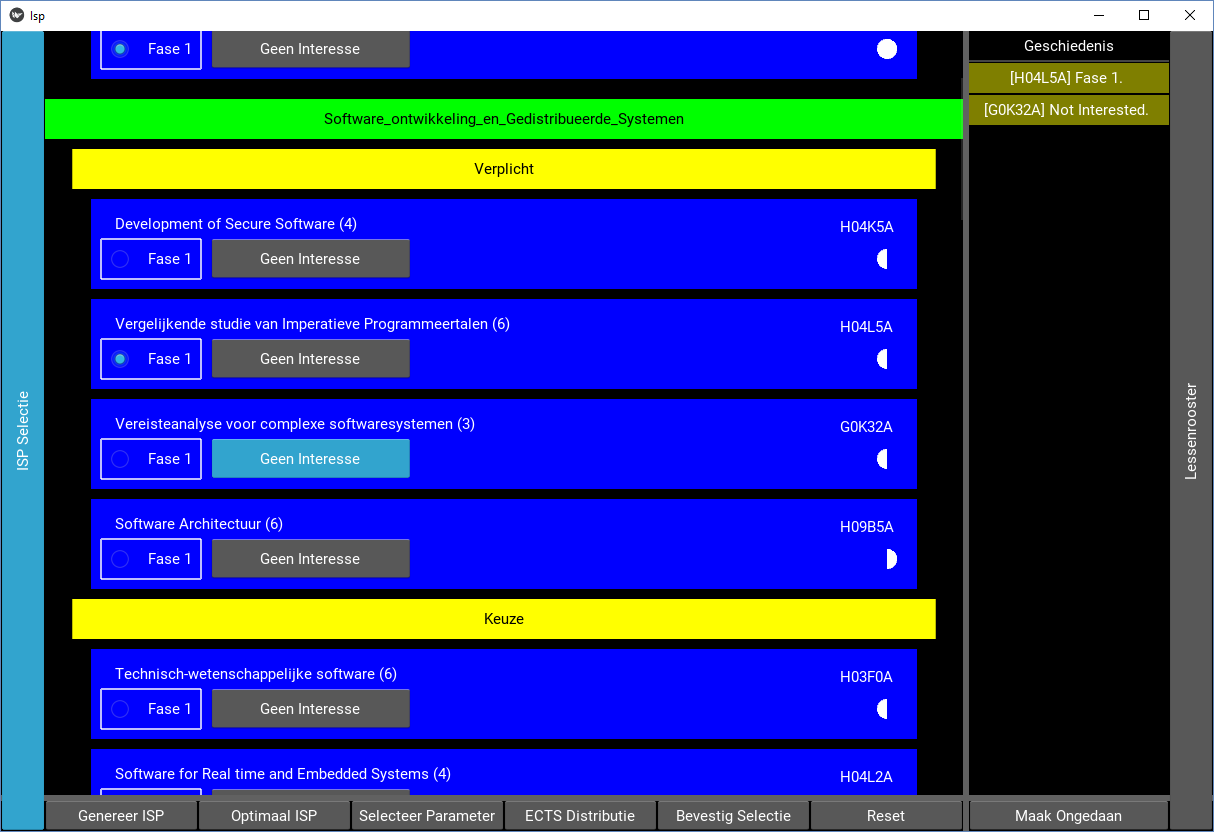
\includegraphics[scale=.5]{sc1.png}
\end{figure}

\paragraph{Overzicht lessenrooster} 
E\'{e}n van de doelstellingen in dit onderzoek is de integratie van het lessenrooster bij het opstellen van het ISP. Het tweede onderdeel van de interface is speciaal hiervoor ontworpen. Voor de huidige selectie van de student zal telkens het bijhorende lessenrooster worden bepaald. In dit onderdeel van de applicatie kan de gebruiker een duidelijk overzicht bekijken van dit lessenrooster en eventuele overlap in lesmomenten laten berekenen. Via de kalender kan de student de dagindeling van eender welke werkdag bekijken. Deze staat weergegeven aan de rechterzijde van het scherm. De knop 'Statistics' onderaan rechts berekent de totale overlap van lesmomenten per week.

/*INSERT SCREENSHOT*/


\subsection{Communicatie tussen Front- en Back-end}
Niet alleen is de syntax tussen IDP en Python compleet verschillend, het zijn ook twee verschillende klassen van programmeertalen respectievelijk declaratief en objectgeori\"{e}nteerd. Dus communicatie tussen de twee talen is niet vanzelfsprekend. Een Python API die toelaat IDP te gebruiken is reeds ontwikkeld \citep{vennekens2015lowering}. Het doel van de API is om de kloof tussen de declaratieve omgeving van IDP en Python kleiner te maken. Door een populaire programmeertaal te kiezen hoopt de auteur dat informatici met een achtergrond in declaratieve talen en logica sneller van IDP gebruik zullen maken zelfs als ze de syntax van IDP niet meester zijn. Persoonlijk heb ik wel al ervaring met IDP en heb dus geopteerd om geen gebruik te maken van de API. 

De input van IDP is compleet tekstueel, de front-end moet een volledig tekst-bestand genereren in een formaat dat IDP kan begrijpen. De output van IDP is opnieuw een tekst-bestand dat de front-end zal moeten parsen om het resultaat te kunnen verwerken. Zo'n tekst-bestand heeft altijd dezelfde opmaak, het bevat een theorie, vocabularium, structuur, procedure en eventueel termen in geval van minimizatie. De front-end bevat een parser object dat voor elke oproep zo'n tekst bestand zal opbouwen. De theorie, vocabularium en de procedures zijn altijd dezelfde en hoeven slecht \'{e}\'{e}nmalig ingelezen te worden. Enkel de structuur zal bij elke nieuwe actie gedeeltelijk dynamische gegenereerd moeten worden. De predicaten in het vocabularium zijn opgedeeld in twee verzamelingen. De eerste verzameling $\Gamma$ bevat de predicaten die vooraf gegeven zijn en gekend zijn door het systeem. Anders gezegd bestaat er een interpretatie G voor $\Gamma$. De andere verzameling $\Omega$, zijn de predicaten waar nog geen interpretatie W voor gegeven is en die door de gebruiker (in dit geval de student) ingevuld zullen moeten worden. Tot deze laatste groep behoren volgende predicaten: Geselecteerd(Vak,Fase) en NietGeinteresseerd(Vak). De bedoeling is om een invulling te zoeken zodat W $\cup$ G consistent is met alle regels van de theorie T.